\chapter{Lecture 10 - Legendre's Equation}
\label{ch:lec10}
\section{Objectives}
The objectives of this lecture are:
\begin{itemize}
\item Illustrate the use of the power series method to solve Legendre's equation. 
\item Introduce some of the properties of Legendre polynomials.
\end{itemize}

\section{Legendre's Equation} \index{Legendre's equation}
The following 2\textsuperscript{nd}-order linear, homogeneous ODE is known as Legendre's equation:
\begin{equation}
\left(1-x^2 \right)u^{\prime \prime}-2xu^{\prime} + m(m+1)u = 0 
\label{eq:legendre}
\end{equation}
where $m$ is a constant.

\newthought{First we will} put Equation \ref{eq:legendre} into standard form:
\begin{equation*}
u^{\prime \prime} - \frac{2x}{\left( 1-x^2 \right)}u^{\prime} + \frac{m(m+1)}{\left(1-x^2 \right)}u = 0
\end{equation*}
We should immediately note that $P(x) = \frac{2x}{\left( 1-x^2 \right)}$ and $Q(x) = \frac{m(m+1)}{\left(1-x^2 \right)}$ are singular (and thus not analytic) at $x=\pm1$. Recall from Theorem \ref{thm:existence-of-power-series-solutions} that $P(x)$ and $Q(x)$ must be analytic for power series solutions to exist.
\newthought{We will restrict} our attention to the interval $x \in (-1,1)$ and use the power series method to find a solution.  Inserting our assumed power series solution into Equation \ref{eq:legendre} gives us:
\begin{fullwidth}
\begin{align*}
\left(1-x^2 \right)\sum\limits_{n=2}^{\infty} n(n-1)c_nx^{n-2} - 2x\sum\limits_{n=1}^{\infty} n c_nx^{n-1} + m(m+1)\sum\limits_{n=0}^{\infty}c_nx^n & = 0 \\
\underbrace{\sum\limits_{n=2}^{\infty}n(n-1)c_nx^{n-2}}_{x^0} - \underbrace{\sum\limits_{n=2}^{\infty}n(n-1)c_nx^n}_{x^2} - \underbrace{\sum\limits_{j=1}^{\infty}2nc_nx^n}_{x^1} + \underbrace{m(m+1)\sum\limits_{n=0}^{\infty}c_nx^n}_{x^0} &= 0
\end{align*}
\end{fullwidth}
where we see that all terms with order lower than $x^2$ need to be pulled outside of their summations so all four can be in phase.
\begin{fullwidth}
\begin{multline*}
(2)(1)c_2 + (3)(2)c_3x + \underbrace{\sum\limits_{n=4}^{\infty}n(n-1)c_nx^{n-2}}_{\substack{k=n-2 \\ n=k+2}} - \underbrace{\sum\limits_{n=2}^{\infty}n(n-1)c_nx^{n}}_{\substack{k=n \\ n=k}} - (2)(1)c_1x - \underbrace{\sum\limits_{n=2}^{\infty}2nc_nx^n}_{\substack{k=n \\ n=k}} + \dots \\
m(m+1) \left(c_0 + c_1x\right) + m(m+1)\underbrace{\sum\limits_{n=2}^{\infty}c_n x^n}_{\substack{k=n \\ n=k}} = 0
\end{multline*}
Combining terms outside of the summations and making the indicated substitutions to combine the summations we get:
\begin{multline*}
\left[m(m+1)c_0 + 2c_2 \right] + [\underbrace{(m(m+1)-2)}_{(m-1)(m+2)}c_1 + 6c_3]x + \dots \\
\sum\limits_{k=2}^{\infty}[(k+2)(k+1)c_{k+2} \underbrace{- k(k-1)c_k - 2kc_k + m(m+1)c_k}_{(m-k)(m+k+1)c_k}]x^k = 0
\end{multline*}
\end{fullwidth}
Applying the indicated algebraic simplifications leads us finally to:\marginnote{\textbf{Note:} Obviously this is a tedious business.  Be careful and make sure you understand each manipulation.}
\begin{multline*}
[m(m+1)c_0+2c_2] + [(m+1)(m+2)c_1 + 6c_3]x + \cdots \\
\sum\limits_{k=2}^{\infty}[(k+2)(k+1)c_{k+2} + (m-k)(m+k+1)c_k]x^k=0
\end{multline*}
The next steps are to find formulas for the power series coefficients, $c_n$, so that the combined coefficient for each power of $x$ in the equation above equals zero. For the constant term $(x^0)$ we have:
\begin{equation*}
c_2 = \frac{-m(m+1)c_0}{2}
\end{equation*}
For the linear term $(x^1)$ we get:
\begin{equation*}
c_3 = \frac{-(m-1)(m+2)}{6}c_1
\end{equation*}
For all other powers of $x$, we get a 2-term recurrence:
\begin{equation*}
c_{k+1} = \frac{-(m-k)(m+k+1)}{(k+2)(k+1)}c_k
\end{equation*}
\begin{margintable}
\begin{tabular}{l}
$k=2$ \\
$c_4 = \frac{-(m-2)(m+3)}{(4)(3)}c_2 = \frac{(m-2)(m+3)m(m+1)}{(4)(3)(2)}c_0$ \\
$k=3$ \\
$c_5 = \frac{-(m-3)(m+4)}{(5)(4)}c_3 = \frac{(m-3)(m+4)(m-1)(m+2)}{(5)(4)(3)(2)}c_1$ \\
\end{tabular}
\end{margintable}
\noindent Organizing these into two solutions we get:
\begin{align*}
u_1(x) &= c_0\left[1 + \frac{c_2}{c_0}x^2 + \frac{c_4}{c_0}x^4 + \cdots \right] \\
&= c_0 \left[1-\frac{m(m+1)}{2!}x^2 + \frac{(m-2)(m+3)m(m+1)}{4!}x^4 + \cdots  \right] \\
u_2(x) &= c_1\left[x + \frac{c_3}{c_1}x^3 + \frac{c_5}{c_1}x^5 + \cdots \right] \\
&= c_1\left[x - \frac{(m-1)(m+2)}{3!}x^3+\frac{(m-3)(m+4)(m-1)(m+2)}{5!}x^5 + \cdots \right]
\end{align*}
So far what we have is messy but, when dealing with power series solutions, messiness is the order of the day.  One point that we have quietly left to the side is whether or not we expect this (so called) power series solution  to converge.\marginnote{\textbf{Reminder:} If the power series that we purport to be a solution to the differential equation is divergent than we really have nothing.}

One way that we can permanently leave these questions to the side is if $m$ is an integer.  Notice that if $m=0$ or is an even integer,\sidenote{i.e. If $m$ is even then $u_1(x)$ is a polynomial.} $u_1(x)$ terminates with a finite number of terms. Similarly with $u_2(x)$ in the case that $m$ is an odd integer. 

\index{Legendre polynomials}
\newthought{These polynomial solutions}, where $m$ is an integer, are referred to as Legendre polynomials.  Legendre polynomials have several important applications; our primary use for them will be when solving equations in spherical coordinate systems.

\section{Important Properties of Legendre Polynomials}
Legendre polynomials are solutions to Legendre's equation where $m$ is an integer:
\begin{equation*}
\left(1-x^2 \right)u^{\prime \prime} - 2xu^{\prime} + m(m+1)u = 0
\end{equation*}

By convention the leading coefficients are chosen such that Legendre polynomials have a maximum value of 1 on the interval $x\in[-1,1]$.  

\begin{margintable}
\begin{tabular}{c | c}
$P_0(x) = 1$ & $P_1(x) = x$ \\\hline
$P_2(x) = \frac{1}{2}(3x^2-1)$ & $P_3(x) = \frac{1}{2}(5x^3-3x)$ \\
\end{tabular}
\caption{The first four Legendre Polynomials}
\label{tab:Legendre-poly}
\end{margintable}
The first few Legendre Polynomials are shown in the Table \ref{tab:Legendre-poly}. Higher order Legendre polynomials can be constructed using a three-term recurrence relation shown in Equation \ref{eq:legendre-three-term}:
\begin{equation}
(n+1)P_{n+1}(x) - (2n+1)xP_n(x) + nP_{n-1}(x) = 0
\label{eq:legendre-three-term}
\end{equation}

\vspace{4.0cm}

Some other properties include:

\begin{align*}
P_n(-x) &= (-1)^nP_n(x) \\
P_n(1) &= 1 \\
P_n(-1) &= (-1)^n \\
P_n(0) &= 0 \text{ for } n\in{\text{odd}} \\
P_n^{\prime}(0) &=0 \text{ for } n\in{\text{even}}
\end{align*}
\begin{marginfigure}
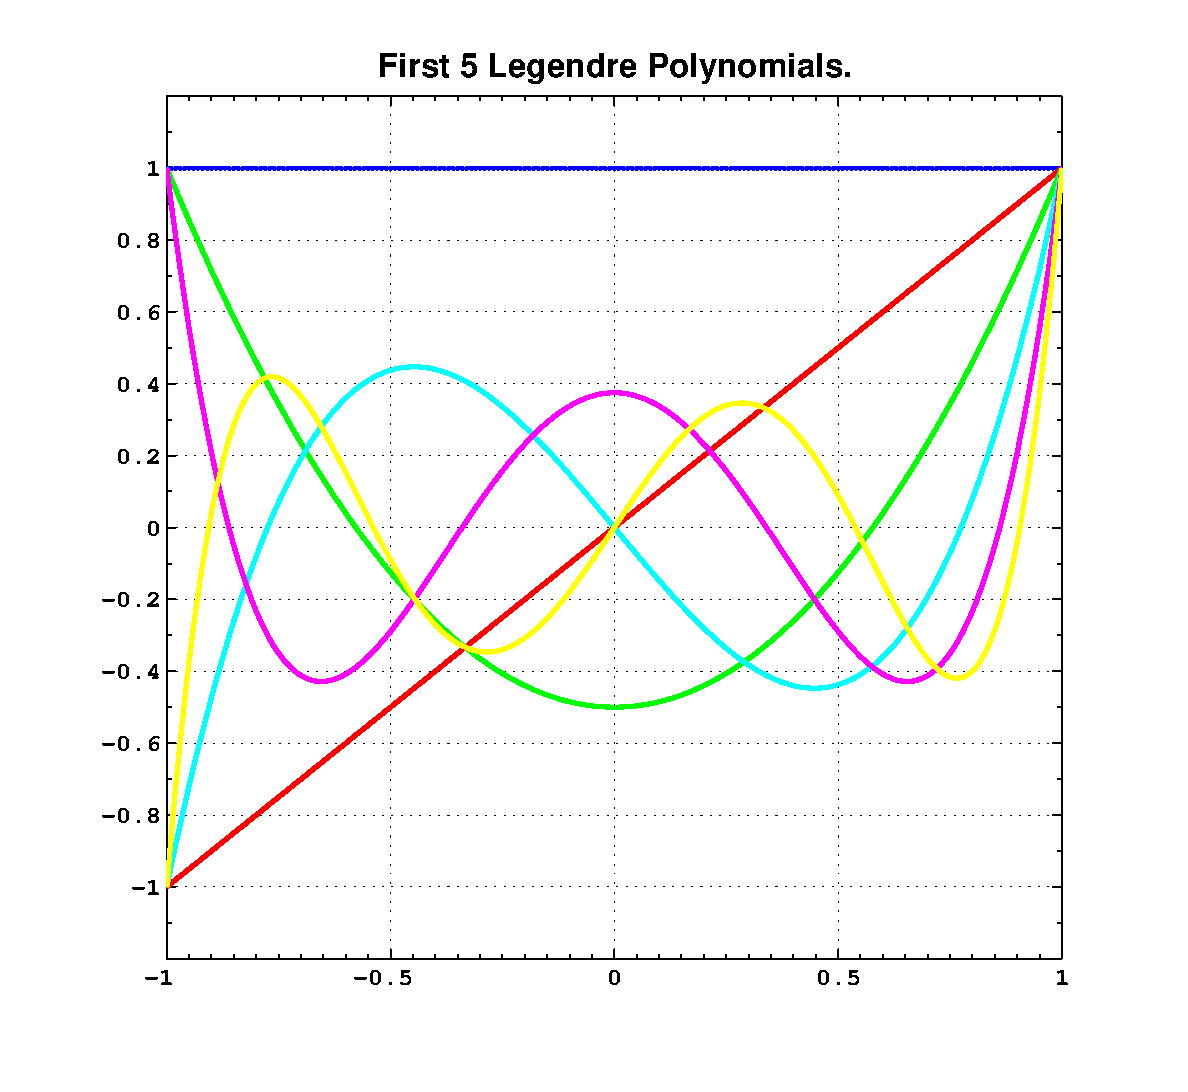
\includegraphics{LegendrePolyPlot.eps}
\caption{Legendre Polynomials of order 0 through 5.}
\label{fig:legendre-poly-plot}
\end{marginfigure}
A plot of the first few Legendre Polynomials is shown in Figure \ref{fig:legendre-poly-plot}.


\newthought{The last property} that we will mention here, and that we will make use of extensively in this course, is the \emph{orthogonality} property of Legendre polynomials.\marginnote[1.0cm]{Orthogonality of functions is analogous to orthogonality of vectors.  Two functions, $f_1(x)$ and $f_2(x)$ are orthogonal on an interval $x\in[a,b]$ if $\int_a^b f_1(x)f_2(x) \ dx = 0$.}
Legendre polynomials are orthogonal over the interval $x \in [-1,1]$.  This mean that Equation \ref{eq:legendre-orthogonality} holds:
\begin{equation}
\int_{-1}^{1} P_n(x) P_m(x) \ dx = 
\begin{cases}
0, \ \ n \ne m \\
\frac{2}{n+1}, \ \ n = m \\
\end{cases}
\label{eq:legendre-orthogonality}
\end{equation}

